\chapter{Definition der Use Cases} \label{Defintion der Use-Cases}
In diesem Kapitel werden die Use Cases für ein Hybrid Cloud-\gls{Deployment} vorgestellt und näher erläutert. Es findet eine Vorauswahl über geeignete technische Komponenten statt, welche anschließend in Kapitel \ref{Umsetzung der Use-Cases und Evaluation} genutzt werden. Weiterhin werden messbare Evaluationskriterien für eine erfolgreiche Umsetzung genannt. Bei Vorauswahl und Evaluationskriterien handelt es sich um in der Praxis übliche Anforderungen im Unternehmensumfeld. Grundlegende Kenntnisse v.a. über IPv4(-Routing), \gls{VPN} und Building Blocks der Public Cloud-Plattformen aus dem vorangegangenen Kapitel \ref{Technische_Grundlagen} werden vorausgesetzt.

\section{Use Case 1: Basis Deployment mit Ende-zu-Ende-Konnektivität}\label{base-deployment}
Es wird ein Basis \gls{Deployment} benötigt, um eine grundlegende Integration in die Firmeninfrastruktur zu ermöglichen. So ist die Grundannahme, dass der Kunde bereits Rechenressourcen in Selbstverwaltung (\glqq Private Cloud\grqq{}) besitzt. Weiterhin hat die Integration von Public Cloud-Diensten noch gar nicht oder nur testweise stattgefunden: Es wurden ein paar Maschinen hochgefahren und bestimmte Internetdienste installiert. Über eine tiefergehende Koppelung mit bestehender Infrastruktur hat der Kunde bisher keine Überlegungen angestellt.\\
Eine Hybrid Cloud besteht, wie bereits beschrieben, aus Public und Private Cloud. Da mit den beiden Public Clouds AWS und Azure gearbeitet wird, wäre hier bereits eine Fallunterscheidung notwendig: Private Cloud $\leftrightarrow$ Azure bzw. Private Cloud $\leftrightarrow$ AWS. Um sich diese Fallunterscheidung sparen zu können, soll ein Dreieck ausgerollt werden, bei dem jeder Punkt eine Cloud-Plattform darstellt.
Optimalerweise wird durch dieses \gls{Deployment} auch die Redundanz erhöht: Fällt eine Verbindung aus bspw. zwischen AWS und Azure, so können Datenpakete weiterhin über die Private Cloud geroutet werden.
Der Use Case soll als Grundaufbau für alle weiteren Use Cases dienen und eine Ende-zu-Ende-Konnektivität für alle Teilnehmer garantieren. Das Dreieck aus AWS, Azure und Private Cloud (s. Abb. \ref{grafik:Use-Case-1_Basis_Deployment}) wird fortan als \textit{\gls{Backbone}} bezeichnet.

\begin{figure}[h]
  \centering
  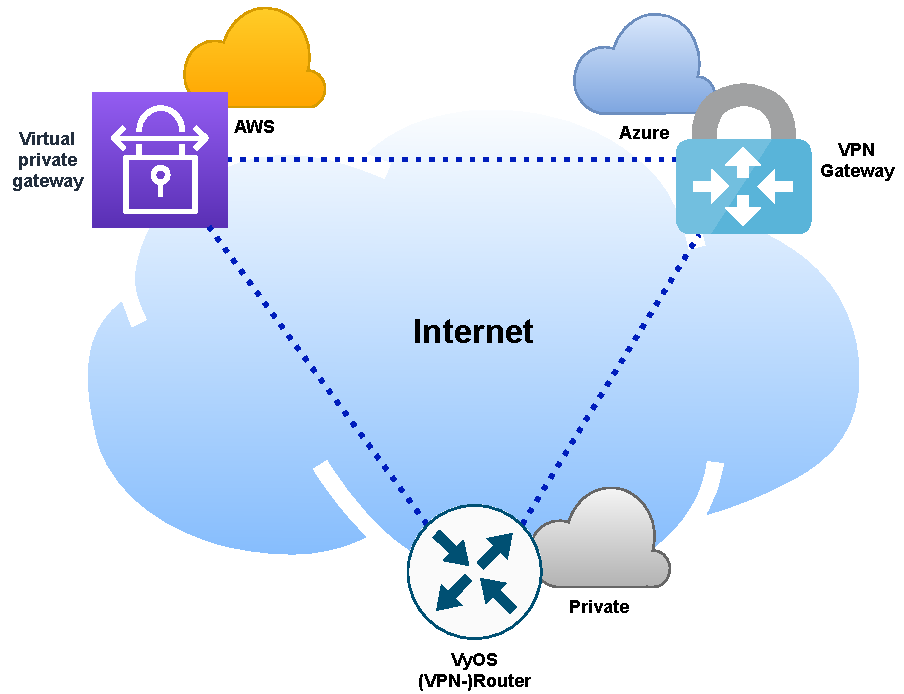
\includegraphics{Figures/Use-Case-1_Basis_Deployment.pdf}
  \caption{Use Case 1: Dreiecks-Topologie für die Hybrid-Cloud (\glqq Backbone\grqq{})}
  \label{grafik:Use-Case-1_Basis_Deployment}
\end{figure}\FloatBarrier

\subsection{Vorauswahl geeigneter technischer Komponenten}
AWS und Azure bieten auf ihren Plattformen Unterstützung für Route-Based \gls{IPsec}-Tunnel\cite[S.32]{awsvpn2021}. Darüber kann eine virtuelle Punkt-zu-Punkt zwischen zwei Standorten hergestellt werden und es kann innerhalb der Tunnel \gls{BGP} gesprochen werden, um ein dynamisches Routing zu ermöglichen\cite[S. 18]{AlShawi2020} \cite[S. 74-79]{Toroman2019}. Gleichzeitig werden übertragene Daten verschlüsselt und dadurch Integrität und Vertraulichkeit geschützt.\\
Das dynamische Routing bietet den Vorteil, dass IPv4-Routen nicht manuell bei allen Gateways des Netzwerks bekannt gemacht werden müssen: Sobald ein Teilnehmer ein neues Netzwerk kennt, wird dies via \gls{BGP} den restlichen Teilnehmern bekannt gegeben.\\
Für das automatisierte \gls{Deployment} der Infrastruktur eignet sich Terraform der Firma Hashicorp. Es besitzt eine Vielzahl an \textit{Resources} (u.a. Azure und AWS), welche es ermöglichen, Infrastrukturkomponenten \textit{reproduzierbar} bereitzustellen.\\
Darüber hinaus wird ein \gls{IPAM} benötigt zur IPv4-Adressverwaltung. Die automatische Zuteilung von Adressbereichen darf nicht dazu führen, dass Adressbereiche mehrfach verteilt werden oder sich Adressbereiche überlappen. Gewählt wurde hier das Werkzeug phpIPAM\cite{phpipam2020}: Es lässt sich sehr gut mit Terraform integrieren, da ein entsprechender Provider zur Verfügung steht\cite{phpipamtf2020}.\\
Die \gls{VPN-Gateway}s, die das \gls{Backbone} aufspannen, sind mit \textit{Virtual private gateway} bei AWS und \textit{VPN Gateway} bei Azure gesetzt. Dies sind die typischen \textit{Building-Blocks}, die von den Cloud-Providern für \gls{VPN}-Verbindungen angeboten werden. Nur wenn sich im Laufe der Arbeit herausstellen sollte, dass diese Systeme nicht interoperabel sein sollten, wird versucht, Alternativen zu finden.\\
Als Router, der die Private Cloud repräsentiert, wurde ein VyOS Router gewählt. Dieser steht als Open Source zur Verfügung, es gibt allerdings auch bezahlten Support für Produktionsumgebungen. Der Router hat \gls{IPsec}- und \gls{BGP}-Unterstützung und besitzt ein Command Line Interface (CLI), über das Konfigurationen getätigt werden können. Eine REST-API steht ebenso zur Verfügung, aber diese ist zum Stand der Bachelor-Arbeit \textit{cutting edge} und wenig dokumentiert\cite{vyosapi2021}. Ein nativer Terraform Provider steht nicht zur Verfügung.\\
Es soll pro Public Cloud eine virtuelle Maschine bereitgestellt werden, um die Ende-zu-Ende-Konnektivität zwischen den Standorten zu verifizieren.
Die Annahme ist, dass der VyOS-Router, das \gls{IPAM} und eine virtuelle Maschine zum Testen in der Private Cloud bereits vorhanden sind. Diese Komponenten sind nicht Teil des (Terraform-)Deployments. Allerdings müssen Konfigurationsänderungen zum \gls{Deployment} geschehen.\\
Prinzipiell lassen sich viele Router-Modelle nutzen, insofern die Unterstützung für genannte Techniken (Route-based \gls{IPsec}, \gls{BGP}) vorhanden ist, bspw. CSR 1000V der Firma Cisco\cite{Durai2016}. Der offene VyOS Router bietet den Vorteil, dass keine Lizenzen für die Nutzung hinterlegt werden müssen, was in vielen Fällen manuelle Konfigurationen erfordert. Außerdem hätten erst einmal passende Lizenzen beschafft werden müssen, was u.U. zu Verzögerungen der Arbeit geführt hätte.
\subsection{Evaluationskriterien}\label{eval-kriterien-uc1}
Nach der Umsetzung wird evaluiert, ob das \gls{Deployment} folgender Kriterien erfolgreich war:
\begin{enumerate}
    \item IPv4-Adressbereiche werden im \gls{IPAM} reserviert und mit AWS \gls{VPC} und Azure \gls{VNET} assoziiert. Test-Szenario: Zur Verifizierung werden die reservierten Adressbereiche mit den assoziierten verglichen.
    \item \gls{IPsec}-Verbindungen werden zwischen allen \gls{VPN-Gateway}s aufgebaut. Test-Szenario: Dies kann mit einem Blick in die verschiedenen \textit{Dashboards} der Cloud-Plattformen bzw. \gls{CLI}-Kommando (VyOS) verifiziert werden.
    \item \gls{BGP}-Sessions werden etabliert und Präfixe zwischen den Teilnehmern ausgetauscht. Die Routen müssen in der Routing-Tabelle sichtbar sein. Test-Szenario: Eine Testmaschine pro Cloud-Standort und Ping-Tests zwischen den Standorten veranlassen.
    \item Die Präfixe sollten im Normalfall über verschiedene \gls{AS}-Pfade sichtbar sein. Nur bei Verbindungsverlust sind Präfixe ausschließlich über einen \gls{AS}-Pfad zu sehen. Test-Szenario analog zu Punkt 2.
    \item Verifizierung der Ende-zu-Ende-Konnektivität und einfache Bandbreitenmessungen. Test-Szenario: Ping-Tests und iPerf3-Messungen zwischen den Standorten.
\end{enumerate}
